%!TEX root=main.tex

\section{Approach}\label{sec:approach}

\subsection{Generation of Pedestrian Trajectories in Simulation}
To compare the capability of humans and machines to predict pedestrian behavior, we have created a simulation of pedestrian behavior. For fairness, the simulation was designed to display the same information to human participants and the models.~\Cref{fig:ped_sim} shows multiple frames of pedestrian trajectories from the bird's eye view.

The simulation implements a dynamics model of pedestrians. Two pedestrians (orange and blue dot) are spawned with a random $x-y$ position and heading angle. The simulation assumes constant velocity $1m/s$, which is a common choice in pedestrian simulations~\cite{Sean2014}. The velocity is used to propagate the position of both agents over time with step size $0.2s$. The positions of both pedestrians are propagated over a maximum of 20 steps until an episode ends. The simulation records a collision label, when the distance of both pedestrians is smaller than the sum of their radius (circumference of the orange and blue circle). 

The simulation uses Reciprocal-Velocity-Obstacles (RVO2)~\cite{Vandenberg2008} as pedestrian dynamics model. Intuitively, each RVO2 pedestrian observes the other pedestrian's position and assumes that they will continue with their current heading and velocity forever. Based on this prediction, the RVO2 pedestrian chooses it's future path the way, that it is as close as possible to its' preferred path, but will never collide with the other agent. Because RVO2 guarantees that no pedestrians will collide, if they all follow RVO2, we have eliminated the possibility for the RVO2 pedestrians to adapt their velocity. This caused approximately 25\% collisions among all episodes.

Reciprocal Velocity Obstacles (RVO2)~\cite{Vandenberg2008} is a decentralized collision avoidance policy and has also been used in other works as pedestrian simulator~\cite{Bera2017}. In comparison to the social forces model~\cite{Helbing1998}, we have decided for the decentralized model RVO2. Decentralized, in this case, means that each pedestrian cannot directly observe the other pedestrian hidden states. We believe in the model being more realistic, because humans also decide about their future trajectory in a decentralized manner. 

RVO2 provides a collaboration coefficient $\alpha$ with determines how "aggressive" or "stubborn" a pedestrian behaves, i.e. it determines how much the pedestrian goes out of the way of the other pedestrian. In this works the parameter is set to the default $0.5$, but future works infers this parameter from real pedestrian data via Bayesian Inference, as demonstrated in~\cite{Bera2017}.

Two datasets have been generated. The first contains $89$ episodes with two pedestrians x-y position and heading over time. The dataset is used for the collection of intent estimation by humans and the HMM. The second dataset contains $8.5$k episodes without pictures and is used by the neural network model.

\begin{figure}[t]
  \centering
  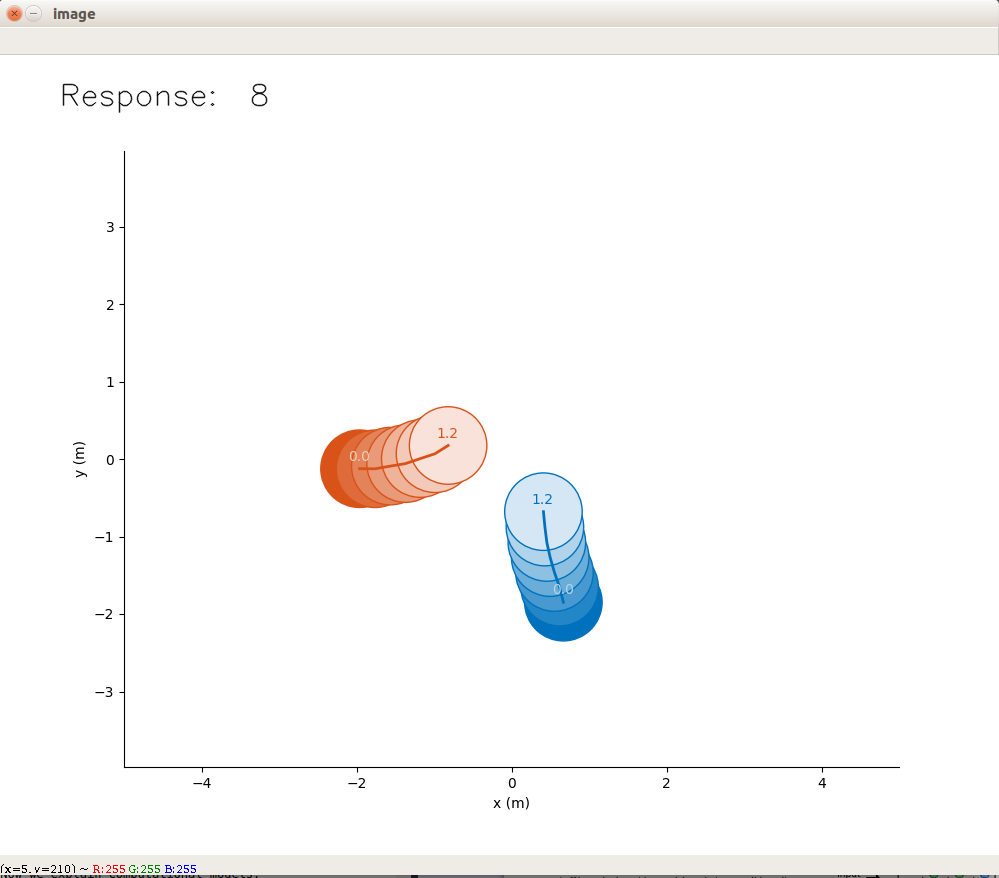
\includegraphics[width=\linewidth]{figures/screenshot.png}
  \caption{A screenshot of human data collection. Each frame shows the trajectories of the two agents by the color gradient (where the lighter color implies the most recent). 
  After participants see a sequence of $5$ frames, they predict pedestrian intent. They do so by entering a rating from $0$ to $10$ which indicates their confidence in the prediction that the two pedestrians are going to collide.}
  \label{fig:human-data-collection}
\end{figure}

\subsection{Collection of Intent Estimation by Humans}
We have asked our participants the following question: \textit{``Assume two normal pedestrians. Normal as in they are ``partially'' cooperative and social pedestrians. Look at the following sequence of $5$ image frames that display two pedestrians' positions over time from the bird's eye view.
Now, how confident are you that the pedestrians' will collide in the near future ($15$ image frames)? Rate from $0$ to $10$ that describe your estimation ($0$: certainly no collision, $10$: certainly collision)''}. 
Our purpose of the question is to give a prior to our participants such that the two pedestrians in the simulator tend to avoid each other but not always (as the word ``partially'' implies). 

\Cref{fig:human-data-collection} shows a screenshot of a simple graphical user interface (GUI) that we have used to collect human data.
Each frame shows the two agents' trajectory, so participants do not need to go back or remember where robots were in the past frames. 
After our participants see the first five frames, they enter their rating from $0$ to $10$, where their responses are saved. 
With this procedure, we collected total $89$ human data samples from three individuals from scientific background. During simulation 24 of these samples have led to a collision, which induces a data set bias towards predicting no collision.
% \\
\\
\subsubsection{Analysis on Collected Human Data} 
\Cref{fig:histogram-human-data} shows the histogram of the ratings.
Interestingly, the histogram shows a bias towards the no collision ratings (i.e., rating $0$).
This might not only be caused by the dataset bias, but also by the question that participants read. 
Because the question mentions about the cooperative and social behaviors of pedestrians, people would have thought that two pedestrians are likely to avoid each other. The histogram reflects this biased prior. 
The data also shows two local maxima at scores $0-3$ and $4-8$ indicating that humans are more confident in prediction no collision than they are in predicting a collision. A possible explanation for this trend is the following: No collision ratings are very confident if the two pedestrians move in opposite directions, as seen in~\cref{fig:sim_no_coll}. When two pedestrians move in the direction of each other as seen in~\cref{fig:sim_coll}, the human prediction is less clear. 
\begin{figure}[t]
  \centering
  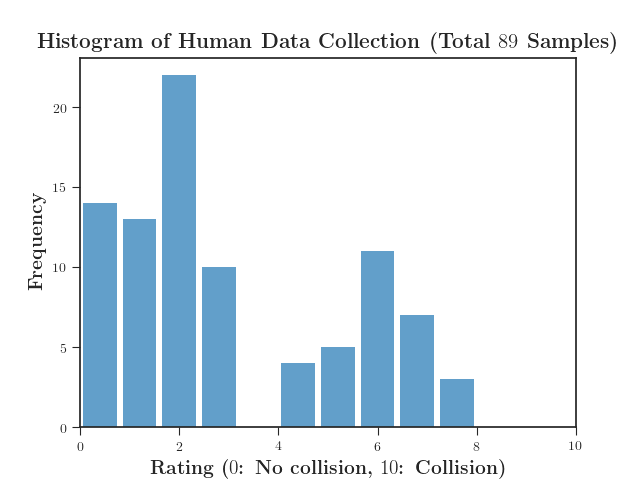
\includegraphics[width=\linewidth]{figures/human_hist.png}
  \caption{Histogram of Participants Ratings. 
  The histogram plots the frequency of the humans' predicted collision probability scores $[0,9]$ on $89$ samples. The histogram shows two peaks towards the no collision rating and a score around $6$. The biased question prior and the dataset bias could partly explain the bias towards the no collision rating. The simulation's ambiguity in a collision case as seen in~\cref{fig:sim_coll}, could explain lack of confidence in a human prediction towards collisions.}
  \label{fig:histogram-human-data}
\end{figure}

\subsection{Neural Network}\label{sec:neural-network}
A neural network (NN) model provides a stronger representation power with lots of learning parameters. 
A neural network model is also trained with a train dataset, which the model learns from and learns how to solve a task. 
One might connect the learning of a neural network model with a train dataset with a human learning from his/her previous experiences. 
Motivated by model's computational power and connection with human's prior experiences, we train a neural network (\cref{fig:nn-without-bootstrap}). We evaluate and analysis the model to understand better about human's decision making in the pedestrian intent prediction task.

Although the neural network model predicts a collision probability, it does not output about uncertainty in its prediction.
Uncertainty provides useful information such that we could use to understand what data points that the model is confused. It also provides a new perspective in understanding relationships between the neural network model and human (e.g., whether the model is also confused at what humans are unsure about). 
Therefore, we take a further step in the neural network model and measure the uncertainty in its prediction (\cref{fig:nn-with-bootstrap}). 
The uncertainty is measured via bootstrapping~\cite{Osband2016, Lakshmi2016}. 
Intuitively, an ensemble of randomly initialized models is trained on overlapping samples of a training dataset. 
Then, during the testing phase, the sample variance of predictions indicates the uncertainty in the prediction. 

\begin{figure}[t]
	\begin{subfigure}[t]{1\linewidth}
		\centering
		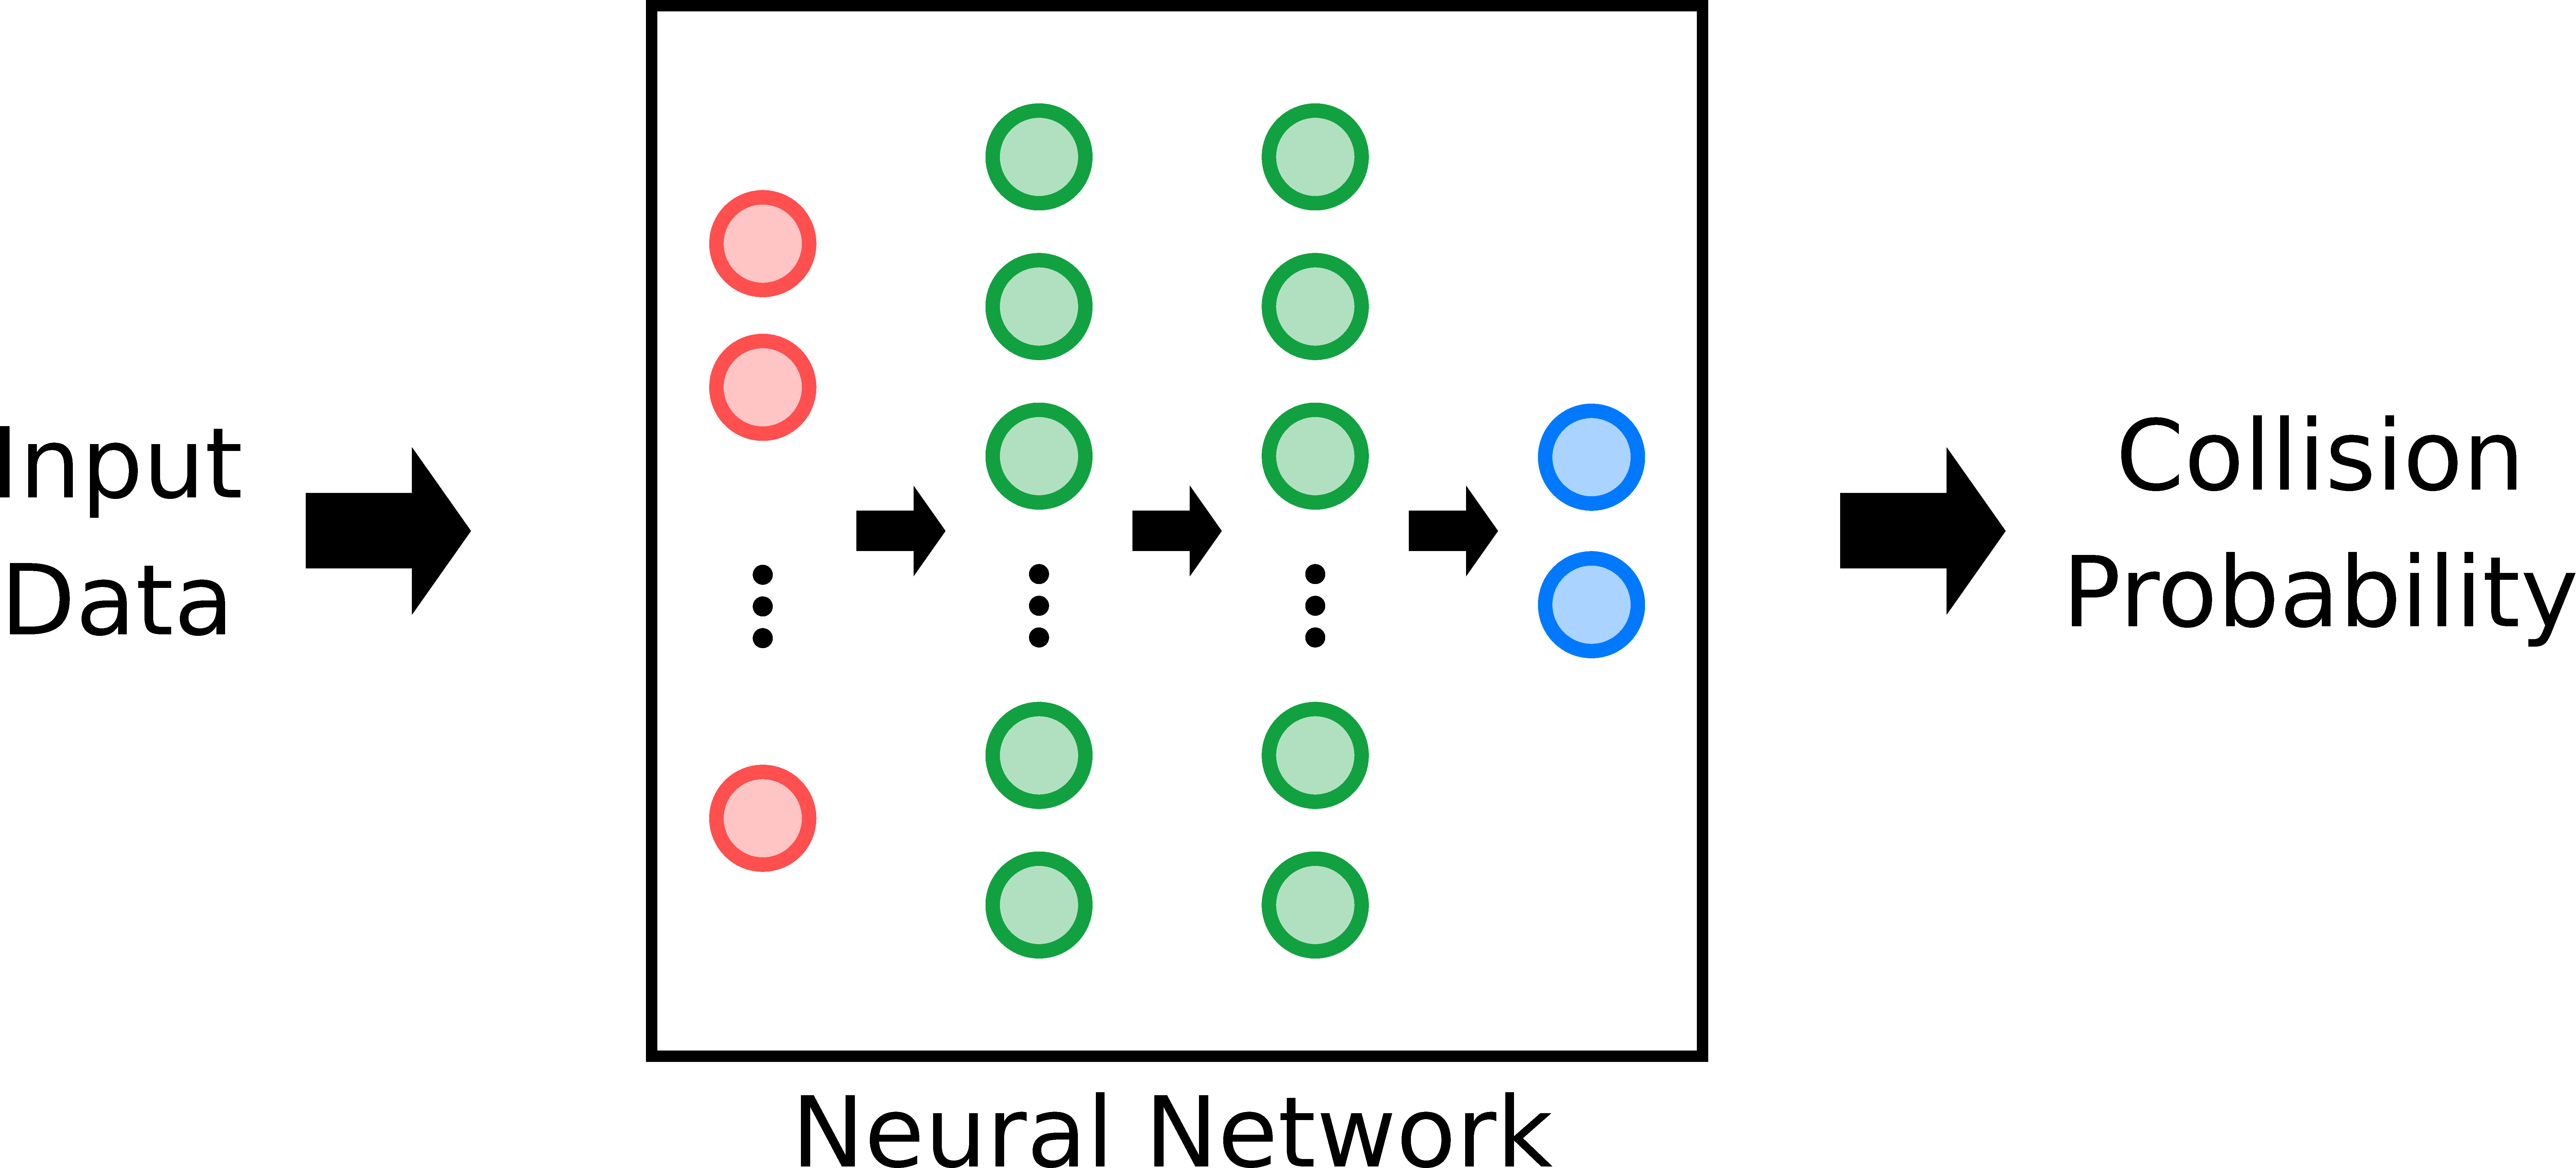
\includegraphics[width=0.95\linewidth]{figures/nn.pdf}
		\caption{Neural Network Model without Bootstrapping.}
		\label{fig:nn-without-bootstrap}
	\end{subfigure}
    \\
    \par\bigskip
	\begin{subfigure}[t]{1\linewidth}
		\centering
		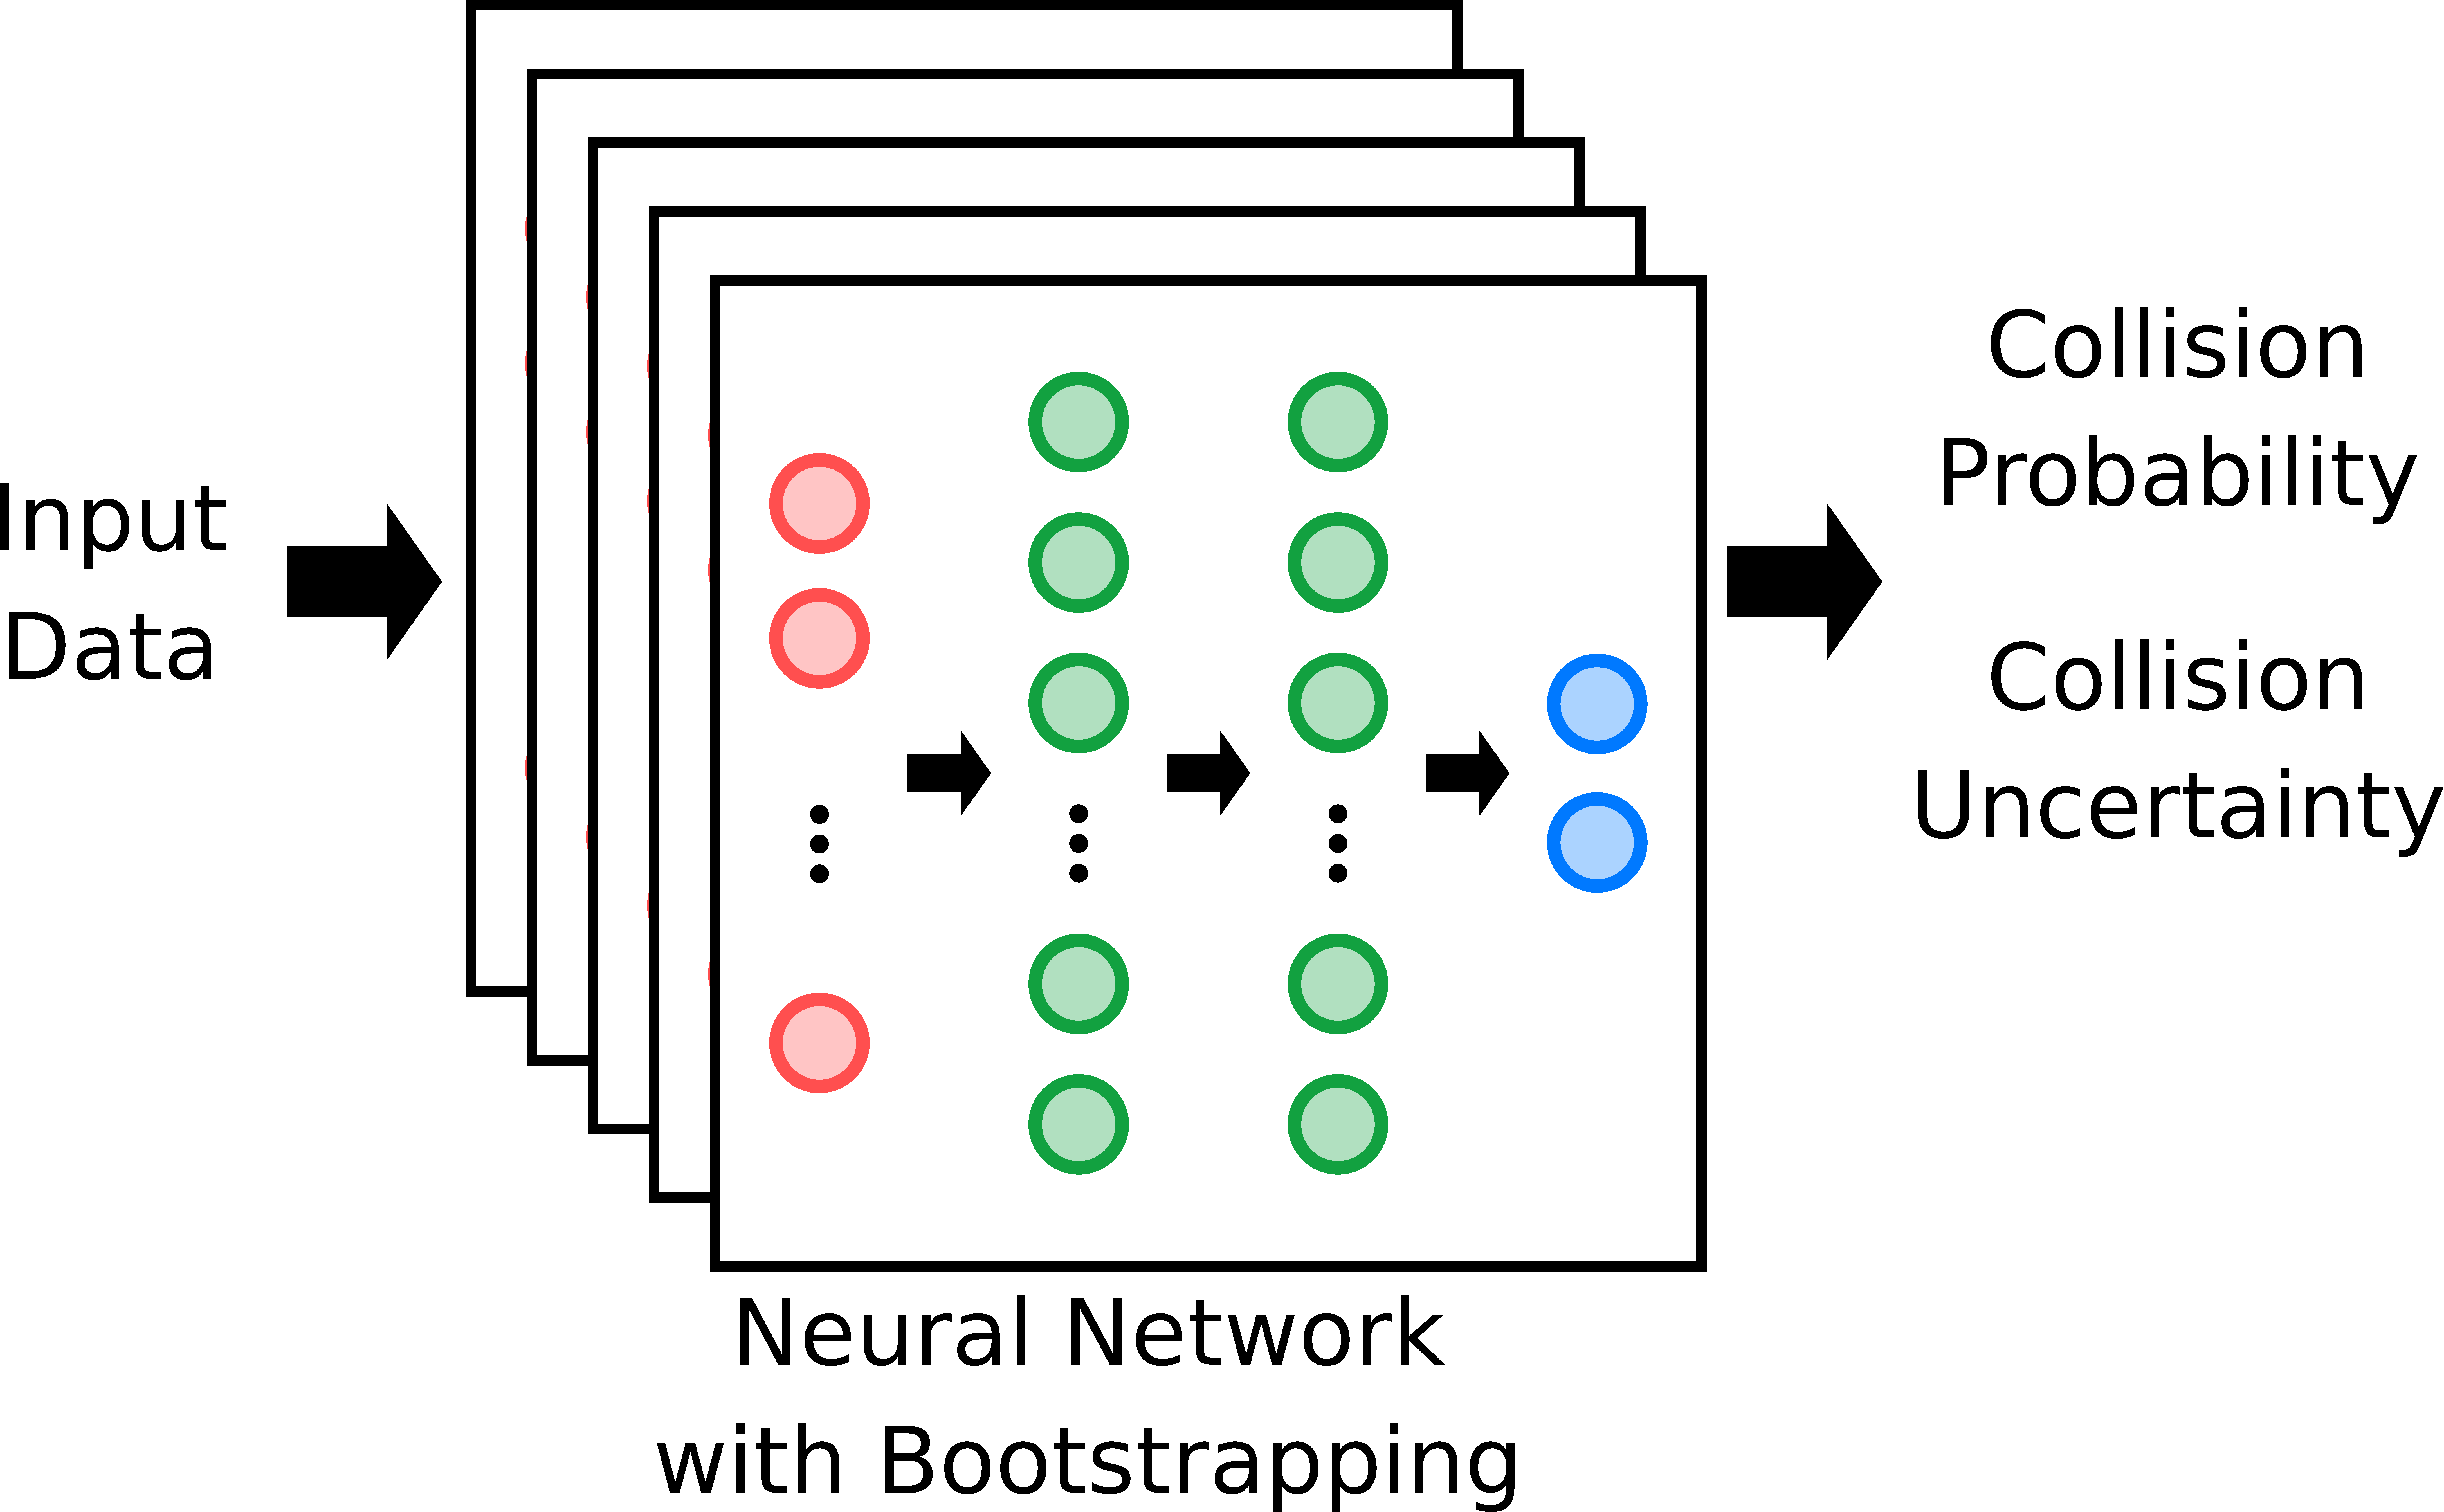
\includegraphics[width=0.95\linewidth]{figures/nn_bootstrap.pdf}
		\caption{Neural Network Model with Bootstrapping.}
		\label{fig:nn-with-bootstrap}
	\end{subfigure}
	\caption{Our two approaches for neural networks. (a) Neural network model with one feed-forward network. (b) Neural network model with Bootstrapping (i.e., ensemble of neural networks) for uncertainty. In (b) the collision probability and uncertainty is the sample mean and variance from the neural network ensemble's predictions.}
	\label{fig:nn-overview}
\end{figure}

\begin{algorithm}[t]
	\caption{Collision Neural Network}
	\label{alg:nn-without-bootstrapping}
	\begin{algorithmic}[1]
	    \Require Train, validation, and test dataset $\mathcal{D}_{train}$, $\mathcal{D}_{val}$, $\mathcal{D}_{test}$
	    \State Initialize a feed-forward neural network model $\mathcal{M}$
	    \State Train the network with train $\mathcal{D}_{train}$ and validation dataset $\mathcal{D}_{val}$
	    \State Test the network with test dataset $\mathcal{D}_{test}$ and get collision probabilities
	\end{algorithmic}
\end{algorithm}

\begin{algorithm}[t]
	\caption{Uncertainty-Aware Collision Neural Network Collision Model}
	\label{alg:nn-with-bootstrapping}
	\begin{algorithmic}[1]
	    \Require Train, validation, and test dataset $\mathcal{D}_{train}$, $\mathcal{D}_{val}$, $\mathcal{D}_{test}$
	    \Require Number of Bootstrapping $N$
	    \State Initialize feed-forward neural network models $\{\mathcal{M}_{1}, \mathcal{M}_{2}, ..., \mathcal{M}_{N} \}$
	    \For{each network $\mathcal{M}_{i}$}
	        \State Randomly shuffle train $\mathcal{D}_{train}$ and validation dataset $\mathcal{D}_{val}$
	        \State Train network $\mathcal{M}_{i}$ 
	    \EndFor
	    \For{each network $\mathcal{M}_{i}$}
	        \State Test network $\mathcal{M}_{i}$ with test dataset $\mathcal{D}_{test}$ and get collision probabilities
	    \EndFor
	    \State Get uncertainty by measuring sample variance in the collision probabilities of $N$ models
	\end{algorithmic}
\end{algorithm}

\begin{figure}[t]
  \centering
  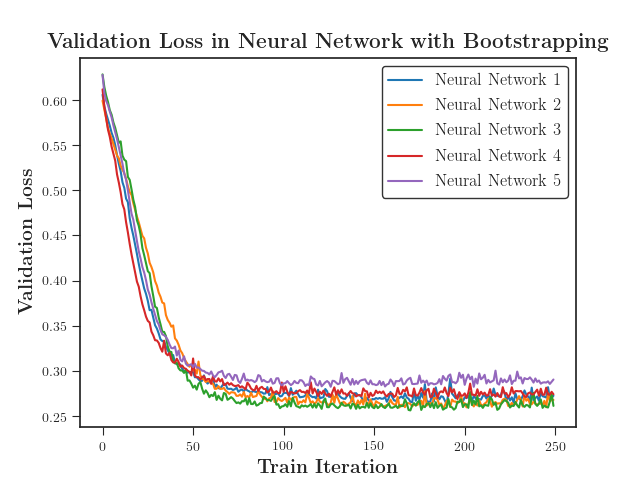
\includegraphics[width=\linewidth]{figures/loss.png}
  \caption{Validation losses for training the neural network with bootstrapping. The validation loss decreases with variances, as desired.}
  \label{fig:ensemble-loss}
\end{figure}

\subsection{Network and Train Details}
Our neural network model is three-layer feed-forward deep neural network, consisting of rectified linear unit (ReLU) activation and $64$ nodes per layer.
A final layer of the softmax activation is used at the output of the policy that provides the collision probability. 
Because our participants only see the locations of two agents, we also provide only location information to the networks. 
Similar to \cite{mnih2015humanlevel}, where they concatenated multiple frames to avoid using a recurrent neural network, we concatenate location information across the first five frames and provide as an input to the network.
Please note that we could also consider using a convolutional neural network to effectively process with image data. 
However, the usage of convolutional layers would cause additional, unnecessary complexities both in learning and understanding between a human and neural network model, which motivated us to experiment based on a feed-forward network.

The (deep) neural networks require lots of data points for learning. 
Thus, from the pedestrian behavior simulation, we collected a sufficient amount of data: $8.5$k trajectories. 
Because collecting human participants' responses on all these data points are expensive, we consider a ground-truth of collision if a collision actually happened during these trajectories.
We divided the dataset with train and validation dataset\footnote{$20$\% of dataset is used as the validation dataset} and trained the neural network models (i.e., neural network model with and without bootstrapping). 
The ensemble size of $5$ is used for the neural network model with bootstrapping. 
The Adam optimizer with a learning rate of $0.0003$ is used. 
The validation data is used to decide to prevent the overfitting. 
\Cref{fig:ensemble-loss} shows the validation losses for the neural network model with bootstrapping. 
The losses are similar but with variances, as desired. 
Pseudocode for neural network model without and with bootstrapping are summarized in \cref{alg:nn-without-bootstrapping} and \cref{alg:nn-with-bootstrapping}, respectively. 

\subsection{Hidden Markov Model}
As black-box neural network alternative, we have implemented a fully introspective Hidden Markov Model (HMM). We thereby make the Markov assumption, i.e. \textit{the future is independent of the past, given the present}. In this case, the future pedestrian intent is independent of previous observations, given the current heading and position observation, and the model. The model's inference of pedestrian intent is converted into a collision prediction and compared and adapted to the humans' predictions. 

\begin{definition}
Formally, a hidden markov model is composed of the following.
\begin{itemize}
    \item a finite set of states $Q = \{q_1, ...,q_n\}$
    \item a transition matrix $A$, such that element $A_{i,j}$ describes the probability of transitioning from state $q_i$ to state $q_j$. 
    \item a finite set of observations $O = \{o_1,...,o_n\}$
    \item an output transition matrix $B$, such that $B_{i,j}$ describes the probability of observation $o_i$ being produced from state $q_j$
    \item an initial probability distribution $\Pi_n$ over the hidden states
\end{itemize}
\end{definition}

\subsection{Hidden Markov Model}
We consider the following structure for formulating collision prediction with a Hidden Markov Model. \\
The simulated data discussed in the prior section gives us information on the position, the speeds, and the orientation of the agent in global space. The underlying stochastic process that is not observable to outsiders is the intention of the agents. The intention of the agents is important in then determining how close they are willing to get, and, thus, the likelihood of collision. \\
Our fundamental problem setup for the HMM was: Given the observation sequence $O_1, O_2,...,O_T$, estimate the optimal sequence of hidden states. \\
Humans only have access to the sequence of relative positions and infer heading and velocity from the short video sequence. Similarly, the HMM only has access to the sequence of relative positions and does not access information about velocity. For model simplicity and a slight advantage, the HMM also accesses the sequence of pedestrian heading angles (i.e. where the pedestrian is looking).
\begin{enumerate}
    \item We place a Gaussian prior on the initially hidden intent. The internal states are discretized action possibilities in the $8$ directions depicted in \label{dir}: north, north-east, east, south-east, south, south-west, west, and north-west.
    \begin{figure}
        \centering
        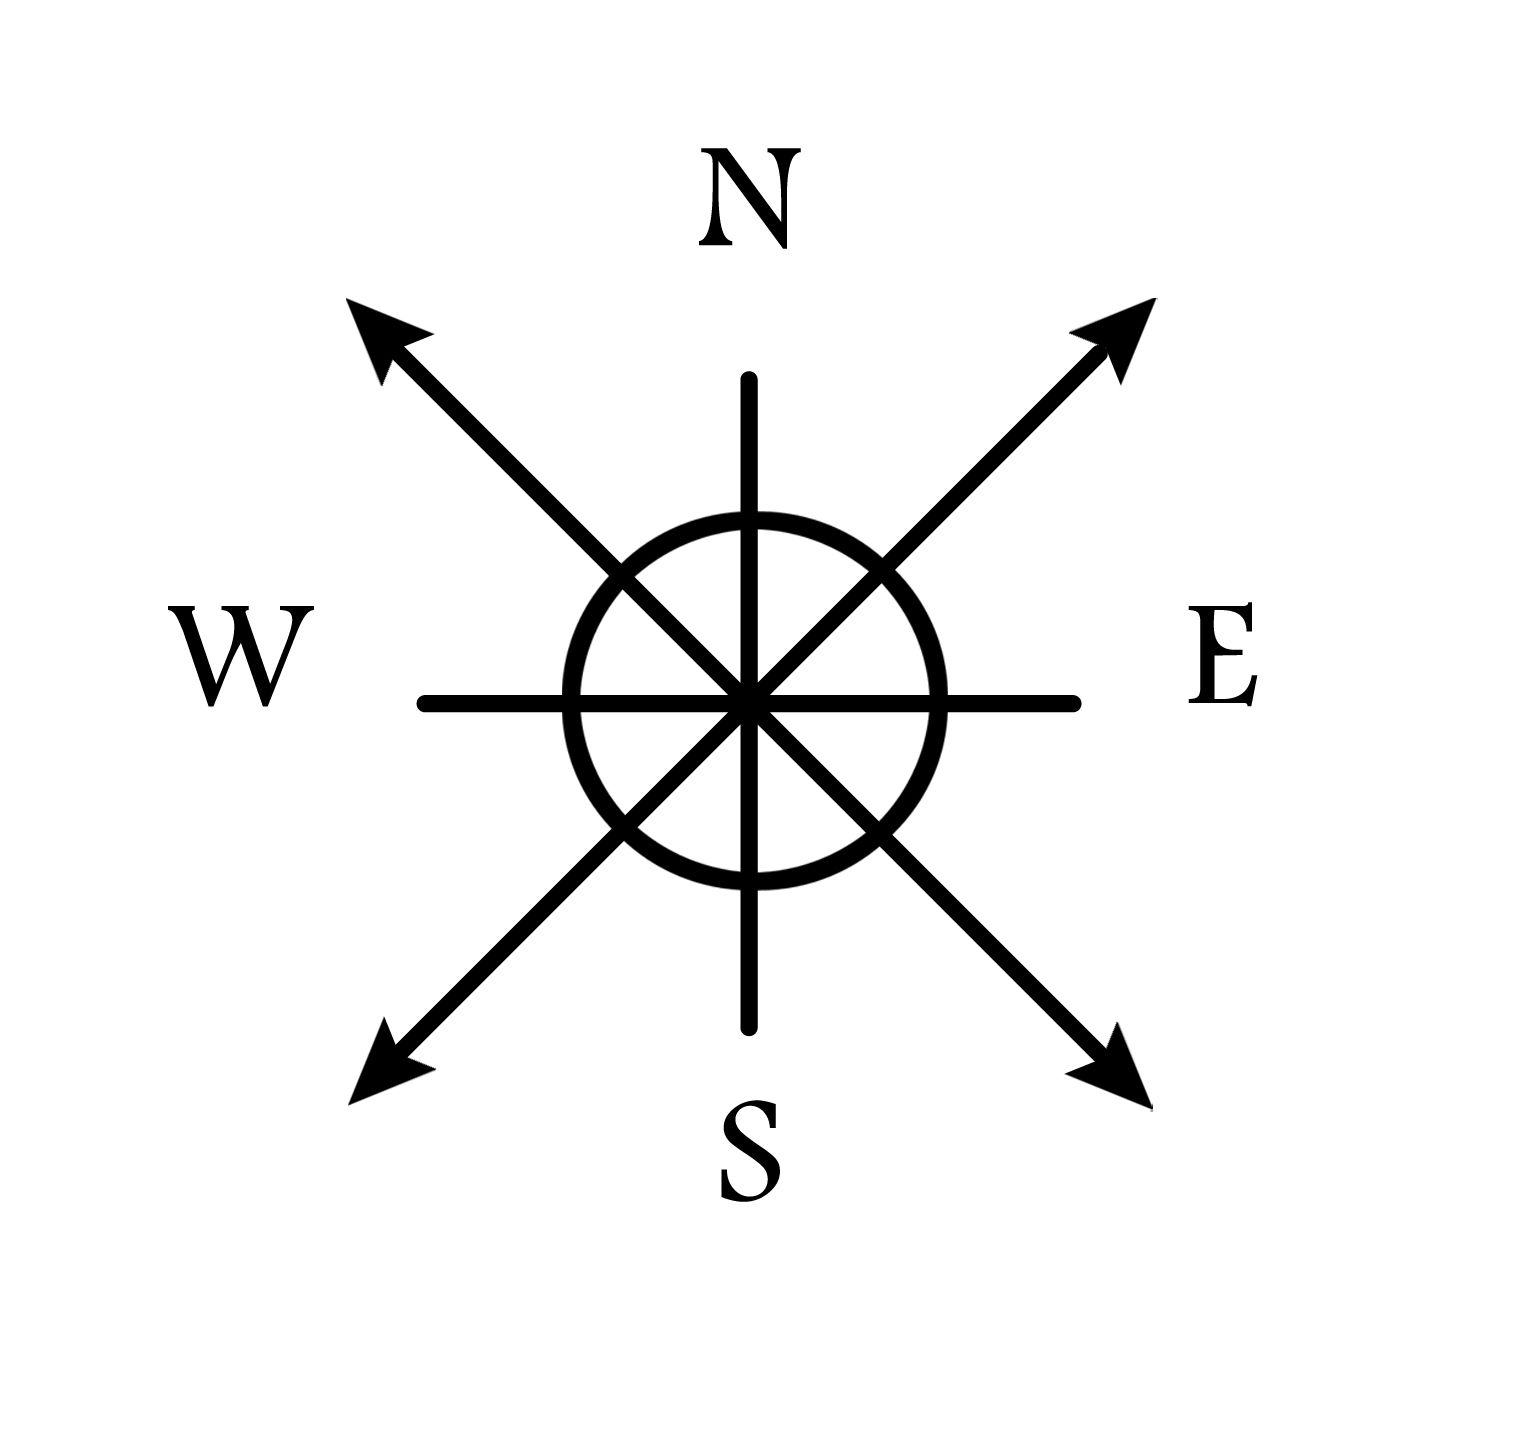
\includegraphics[scale=0.5]{figures/compass.jpg}
        \caption{Considered 8 orientation directions for HMM: north, north-east, east, south-east, south, south-west, west, and north-west.}
        \label{fig:dir}
    \end{figure} \\ 
    \textbf{Note:} Similar to inferring, if a coin is loaded, one could adapt this prior to better match human knowledge. However, this mostly makes sense in domains, where the human has a strong prior about future direction, i.e. in a one-way street. As in our domain all directions can be seen equally likely, we have concentrated on adapting different parameters.
    \item The models are fitted to the first five time steps of observation data from each agent. We then want a sequence of optimal states for future agent actions. 
    The criterion we use to choose the states, $i$, is the state with most likelihood. To implement this solution, we let $\gamma$ be the probability of being in state $q_i$ at time $t+1$, given the observation sequence $O$ and the model $\lambda$.
    $$\gamma_{t+1}(i) = Pr(i_t=q_i|O, \lambda)$$
    We sample the model for the most likely state for the agent's orientation. In other words, 
    $$i_{t+1} = argmax[ \gamma_{t+1}(i)]$$
    \item Given the most likely state for the agent's orientation and the agent's last known position, we can predict the next positions of those agents. 
    \item We use both position models to derive a euclidean distance model between the agents. We calculate the euclidean distance from the position samples in the prior step. We create a euclidean distance model based on the euclidean distances. We define the discrete states of the distance model to range from $[0, 9]$. These are in the original graph units. 
    \item We use the euclidean distance model to then sample for the most likely euclidean distances. Collisions are defined based on a reasonable threshold distance $x$, where if the euclidean distance $d_t$ at time step $t$ is $d_t < x$, we determine there will be a collision. 
\end{enumerate}
